\documentclass{beamer}\usepackage[]{graphicx}\usepackage[]{color}
% maxwidth is the original width if it is less than linewidth
% otherwise use linewidth (to make sure the graphics do not exceed the margin)
\makeatletter
\def\maxwidth{ %
  \ifdim\Gin@nat@width>\linewidth
    \linewidth
  \else
    \Gin@nat@width
  \fi
}
\makeatother

\definecolor{fgcolor}{rgb}{0.345, 0.345, 0.345}
\newcommand{\hlnum}[1]{\textcolor[rgb]{0.686,0.059,0.569}{#1}}%
\newcommand{\hlstr}[1]{\textcolor[rgb]{0.192,0.494,0.8}{#1}}%
\newcommand{\hlcom}[1]{\textcolor[rgb]{0.678,0.584,0.686}{\textit{#1}}}%
\newcommand{\hlopt}[1]{\textcolor[rgb]{0,0,0}{#1}}%
\newcommand{\hlstd}[1]{\textcolor[rgb]{0.345,0.345,0.345}{#1}}%
\newcommand{\hlkwa}[1]{\textcolor[rgb]{0.161,0.373,0.58}{\textbf{#1}}}%
\newcommand{\hlkwb}[1]{\textcolor[rgb]{0.69,0.353,0.396}{#1}}%
\newcommand{\hlkwc}[1]{\textcolor[rgb]{0.333,0.667,0.333}{#1}}%
\newcommand{\hlkwd}[1]{\textcolor[rgb]{0.737,0.353,0.396}{\textbf{#1}}}%
\let\hlipl\hlkwb

\usepackage{framed}
\makeatletter
\newenvironment{kframe}{%
 \def\at@end@of@kframe{}%
 \ifinner\ifhmode%
  \def\at@end@of@kframe{\end{minipage}}%
  \begin{minipage}{\columnwidth}%
 \fi\fi%
 \def\FrameCommand##1{\hskip\@totalleftmargin \hskip-\fboxsep
 \colorbox{shadecolor}{##1}\hskip-\fboxsep
     % There is no \\@totalrightmargin, so:
     \hskip-\linewidth \hskip-\@totalleftmargin \hskip\columnwidth}%
 \MakeFramed {\advance\hsize-\width
   \@totalleftmargin\z@ \linewidth\hsize
   \@setminipage}}%
 {\par\unskip\endMakeFramed%
 \at@end@of@kframe}
\makeatother

\definecolor{shadecolor}{rgb}{.97, .97, .97}
\definecolor{messagecolor}{rgb}{0, 0, 0}
\definecolor{warningcolor}{rgb}{1, 0, 1}
\definecolor{errorcolor}{rgb}{1, 0, 0}
\newenvironment{knitrout}{}{} % an empty environment to be redefined in TeX

\usepackage{alltt}

\usepackage{default}
\usepackage{animate} %need the animate.sty file 
\usepackage{graphicx}
%\graphicspath{{/home/sahir/Dropbox/jobs/laval/minicours/slides/}}
\usepackage{hyperref, url}
%\usepackage[round,sort]{natbib}   % bibliography omit 'round' option if you prefer square brackets
%\bibliographystyle{apalike}
\usepackage{biblatex}
\bibliography{bib.bib}
% Removes icon in bibliography
\setbeamertemplate{bibliography item}[text]

\usepackage[normalem]{ulem}

\setbeamertemplate{theorems}[numbered]

\setbeamertemplate{caption}[numbered]
\setbeamertemplate{caption label separator}{: }
\setbeamercolor{caption name}{fg=normal text.fg}

%\newtheorem{prop}{Proposition}
%\newenvironment{theoremc}[1]
%{\begin{shaded}\begin{theorem}[#1]}
%		{\end{theorem}\end{shaded}}
	
%\newtheorem{examplefirst}{Example}
%\newtheorem{examplesecond}{Example}
%\newenvironment<>{examplefirst}[1][]{%
%	\setbeamercolor{block title example}{bg=lightgray}%
%	\begin{example}#2[#1]}{\end{example}}
%\newenvironment<>{examplesecond}[1][]{%
%	\setbeamercolor{block title example}{fg=white,bg=blue!75!black}%
%	\begin{example}#2[#1]}{\end{example}}	

%\usepackage{amsthm}


\usepackage[figurename=Fig.]{caption}
\usepackage{subfig}
\usepackage{tikz, pgfplots,epsfig}
\usetikzlibrary{arrows,shapes.geometric}
\usepackage{color, colortbl,xcolor}
\definecolor{lightgray}{RGB}{200,200,200}
\definecolor{palegray}{RGB}{221,221,221}
\definecolor{myblue}{RGB}{0,89,179}
\definecolor{myorange}{rgb}{0.776,0.357,0.157}

\definecolor{gray}{RGB}{110,110,110}
\definecolor{darkgray}{RGB}{100,100,100}
\definecolor{lightgray}{RGB}{200,200,200}
\definecolor{turquoise}{RGB}{81,193,188}
\definecolor{tomato}{RGB}{255,136,136}
\definecolor{mandarina}{RGB}{229,169,25}
\definecolor{foreground}{RGB}{81,141,193}
\definecolor{background}{RGB}{246,244,240}
\definecolor{highlight}{RGB}{229,169,25}
\definecolor{lowlight}{RGB}{200,200,200}
\definecolor{beige}{RGB}{255,255,240}
\definecolor{pinkish}{RGB}{255,223,247}

\newcommand{\code}[1]{\texttt{#1}}


\usepackage{comment}
\setbeamercolor{frametitle}{fg=myblue}
\setbeamercolor{section in head/foot}{bg=myblue, fg=white}
\setbeamercolor{author in head/foot}{bg=myblue}
\setbeamercolor{date in head/foot}{bg=myblue}

\usepackage{amsthm}
\usepackage{shadethm}
%\colorlet{shadecolor}{blue!15}
\colorlet{shadecolor}{palegray}
%\setlength{\shadeboxrule}{.4pt}

%\newshadetheorem{thm}{Theorem}
\newshadetheorem{defm}{Definition}
\newshadetheorem{exm}{Exercise}
\newshadetheorem{remarkm}{Remark}
%\definecolor{shadethmcolor}{HTML}{EDF8FF}
\definecolor{shadethmcolor}{RGB}{221,221,221}
%\definecolor{shaderulecolor}{HTML}{45CFFF}
\definecolor{shaderulecolor}{RGB}{0,89,179}
\setlength{\shadeboxrule}{.4pt}

\newtheorem{thm}{Theorem}
\newcommand{\statetheoremhoriz}[2][\textwidth]{
	\par\noindent\tikzstyle{mybox} = [draw=myblue,left color=cyan!50,
	right color=cyan!5,thick,rectangle,inner sep=6pt]
	\begin{tikzpicture}
	\node [mybox] (box){%
		\begin{minipage}{#1}{#2}\end{minipage}
	};
	\end{tikzpicture}
}
\newcommand{\statetheoremvert}[2][\textwidth]{
	\par\noindent\tikzstyle{mybox} = [draw=myblue,top color=cyan!50,
	bottom color=cyan!5,thick,rectangle,inner sep=6pt]
	\begin{tikzpicture}
	\node [mybox] (box){%
		\begin{minipage}{#1}{#2}\end{minipage}
	};
	\end{tikzpicture}
}
\newcommand{\statetheoremsolid}[2][\textwidth]{
	\par\noindent\tikzstyle{mybox} = [draw=myblue,fill=palegray,
	thick,rectangle,inner sep=6pt]
	\begin{tikzpicture}
	\node [mybox] (box){%
		\begin{minipage}{#1}{#2}\end{minipage}
	};
	\end{tikzpicture}
}

\usetikzlibrary{shapes.geometric, arrows,shapes.symbols,decorations.pathreplacing}
\tikzstyle{startstop} = [rectangle, rounded corners, minimum width=3cm, minimum height=1cm, draw=black, fill=pinkish,text width=3.5cm]
\tikzstyle{startstop2} = [rectangle, rounded corners, minimum width=3cm, minimum height=1cm, draw=black, fill=background,text width=4.5cm]
\tikzstyle{startstop3} = [rectangle, rounded corners, minimum width=3cm, minimum height=1cm, draw=black, fill=beige,text width=3.0cm]
\tikzstyle{startstop4} = [rectangle, rounded corners, minimum width=3cm, minimum height=1cm, draw=black, fill=pinkish,text width=4.5cm]
\tikzstyle{io} = [trapezium, trapezium left angle=70, trapezium right angle=110, minimum width=2cm, minimum height=1cm, text centered, draw=black, fill=blue!30,text width=1.5cm]
\tikzstyle{process} = [rectangle, minimum width=1cm, minimum height=1cm, text centered, draw=black, fill=orange!30,text width=2cm]
\tikzstyle{decision} = [diamond, minimum width=2cm, minimum height=1cm, text centered, draw=black, fill=green!30]
\tikzstyle{arrow} = [thick,->,>=stealth]
\tikzstyle{both} = [thick,<->,>=stealth, red]


\usepackage{array}
\newcolumntype{L}{>{\centering\arraybackslash}m{3cm}} % used for text wrapping in ctable
\usepackage{ctable}
\usepackage[utf8]{inputenc}
\usepackage{fontenc}
\usepackage{pifont}% http://ctan.org/pkg/pifont
\newcommand{\cmark}{\ding{51}}%
\newcommand{\xmark}{\ding{55}}%
\def\widebar#1{\overline{#1}}
\definecolor{whitesmoke}{rgb}{0.96, 0.96, 0.96}

\usepackage{amssymb}
\usepackage{amsmath}

\usepackage{bm}
\def\transpose{{\sf{T}}}
\def\E{{\skew0\bm{E}}}
\def\Xvec{{\skew0\bm{X}}}
\def\Xveca{{\skew0\bm{X}}_1}
\def\Xvecb{{\skew0\bm{X}}_2}

\def\Yvec{{\skew0\bm{Y}}}
\def\bmY{{\skew0\bm{Y}}}
\def\bmX{{\skew0\bm{X}}}
\def\bmy{{\skew0\bm{y}}}
\def\bmG{{\skew0\bm{G}}}
\def\bmS{{\skew0\bm{S}}}
\def\bmA{{\skew0\bm{A}}}
\def\bmB{{\skew0\bm{B}}}
\def\bmD{{\skew0\bm{D}}}
\def\bmI{{\skew0\bm{I}}}
\def\bmV{{\skew0\bm{V}}}
\def\bmU{{\skew0\bm{U}}}
\def\bv{{\skew0\bm{v}}}
\def\bw{{\skew0\bm{w}}}
\def\bmm{{\skew0\bm{m}}}
\def\bmzero{{\skew0\bm{0}}}
\def\bx{{\skew0\bm{x}}}
\def\xveca{{\skew0\bm{x}}_1}
\def\xvecb{{\skew0\bm{x}}_2}

\def\N{{\skew0\mathcal{N}}}
\def\T{{\small T}}

\def\mvec{{\skew0\bm{m}}}
\def\bmmu{{\skew0\bm{\mu}}}
\def\muvec{{\skew0\bm{\mu}}}
\def\balpha{{\skew0\bm{\alpha}}}
\def\bbeta{{\skew0\bm{\beta}}}
\def\bmtheta{{\skew0\bm{\theta}}}
\def\btheta{{\skew0\bm{\theta}}}

\def\cvec{{\skew0\mathbf{c}}}

\def\Xbar{\overline{X}}

\definecolor{lightgray}{rgb}{0.91,0.91,0.91}
\definecolor{purpleblue}{rgb}{0.50,0.50,1.00}



\usepackage{fontspec}
%\setsansfont{Fira Sans}
%\setmonofont{Fira Mono}
%\setsansfont[ItalicFont={Fira Sans Light Italic},BoldFont={Fira Sans},BoldItalicFont={Fira Sans Italic}]{Fira Sans Light}
%\setmonofont[BoldFont={Fira Mono Medium}]{Fira Mono}

\def\installpath{/usr/local/share/texmf/fonts/opentype/libertinus/}
\setmainfont{LibertinusSerif}[
UprightFont    = *-Regular,
BoldFont       = *-Bold,
ItalicFont     = *-Italic,
BoldItalicFont = *-BoldItalic,
Ligatures      = TeX,
Extension      = .otf,
Path           = \installpath/
]

\setsansfont{LibertinusSerif}[
UprightFont    = *-Regular,
BoldFont       = *-Bold,
ItalicFont     = *-Italic,
BoldItalicFont = *-BoldItalic,
Ligatures      = TeX,
Extension      = .otf,
Path           = \installpath/
]


\setmonofont{LibertinusSerif}[
UprightFont    = *-Regular,
BoldFont       = *-Bold,
ItalicFont     = *-Italic,
BoldItalicFont = *-BoldItalic,
Ligatures      = TeX,
Extension      = .otf,
Path           = \installpath/
]



\setbeamercolor{itemize item}{fg=myblue}
%\setbeamertemplate{itemize item}[square]
\setbeamertemplate{itemize items}[circle]
%\setbeamertemplate{blocks}[rounded][shadow=true]


%\setbeamertemplate{navigation symbols}{\usebeamercolor[fg]{title in head/foot}\usebeamerfont{title in head/foot}\insertframenumber}


%\setbeamertemplate{footline}{}

\beamertemplatenavigationsymbolsempty % toggle off if you want navigation symbols at the bottom

\setbeamertemplate{footline}
{ \usebeamercolor[fg]{page number in head/foot}%
	\usebeamerfont{page number in head/foot}%
	\hspace{1em}\insertsectionhead%
	\hfill%
	\insertframenumber\,/\,\hyperlinkappendixstart{\insertmainframenumber}
	\ifnum \thepage = \insertframeendpage{\small .}\else{\phantom{\small .}}\fi
	\hspace{1em}
	\vskip2pt%
}

\newtheorem{proposition}[theorem]{Proposition}
\newtheorem{exercise}[theorem]{Exercise}

\titlegraphic{\hfill
\includegraphics[height=1cm]{../mcgill_logo.png}}


%% You also use hyperref, and pick colors 
\hypersetup{colorlinks,citecolor=myorange,filecolor=red,linkcolor=brown,urlcolor=blue}

\newcommand {\framedgraphiccaption}[2] {
	\begin{figure}
		\centering
		\includegraphics[width=\textwidth,height=0.8\textheight,keepaspectratio]{#1}
		\caption{#2}
	\end{figure}
}

\newcommand {\framedgraphic}[1] {
	\begin{figure}
		\centering
		\includegraphics[width=\textwidth,height=0.9\textheight,keepaspectratio]{#1}
	\end{figure}
}


\AtBeginSection[]{
	\begin{frame}
		\vfill
		\centering
		\begin{beamercolorbox}[sep=8pt,center,shadow=true,rounded=true]{title}
			\usebeamerfont{title}\insertsectionhead\par%
		\end{beamercolorbox}
		\vfill
	\end{frame}
}

\newcommand\Wider[2][3em]{%
	\makebox[\linewidth][c]{%
		\begin{minipage}{\dimexpr\textwidth+#1\relax}
			\raggedright#2
		\end{minipage}%
	}%
}


\makeatletter

\def \iqsssectiontitleheader {}

\newcommand{\iqsssectiontitle}[1]{
	\def \iqsssectiontitleheader{#1}
}

\@ifundefined{insertmainframenumber}
{%
	% \insertmainframenumber not defined
	\newcommand{\insertmainframenumber}{\inserttotalframenumber}
}
{%
	% \insertmainframenumber already defined
}%


\AtBeginSection[]{
	\title{\insertsectionhead}
	{
		%\definecolor{white}{RGB}{140,193,250}
		%\definecolor{white}{RGB}{200,200,200}
		%\definecolor{white}{RGB}{242,244,247}
		\definecolor{white}{RGB}{0,89,179}
		%\definecolor{iqss@orange}{rgb}{1,1,1}
		\ifnum \insertmainframenumber > \insertframenumber
		%\setbeamercolor{background canvas}{bg=myblue}
		%\setbeamercolor{normal text}{fg=black,bg=white}
		%\setbeamercolor{frametitle}{fg=red}
		%\setbeamercolor{section in toc}{fg=myblue, bg=white}
		%\setbeamercolor{subsection in toc}{fg=myblue, bg=white}
		\frame{
			\frametitle{\iqsssectiontitleheader}
			\tableofcontents[currentsection]
		}
		\else
		\frame{
			\frametitle{Backup Slides}
			\tableofcontents[sectionstyle=shaded/shaded,subsectionstyle=shaded/shaded/shaded]
		}
		\fi
	}
}
\makeatother

\pgfplotsset{compat=1.16}

%\let\oldShaded\Shaded
%\let\endoldShaded\endShaded
%\renewenvironment{Shaded}{\footnotesize\oldShaded}{\endoldShaded}
\IfFileExists{upquote.sty}{\usepackage{upquote}}{}
\begin{document}



%\title{Introduction to Regression Trees}
%\author{Sahir Bhatnagar \inst{1}}
%\author[shortname]{Sahir Rai Bhatnagar, PhD Candidate (Biostatistics) }
%\institute[shortinst]{Department of Epidemiology, Biostatistics and Occupational Health}

\title{Introduction to Inferential Statistics}
\author{EPIB 607 - FALL 2020}
\institute{
	Sahir Rai Bhatnagar\\
	Department of Epidemiology, Biostatistics, and Occupational Health\\
	McGill University\\
	
	\vspace{0.1 in}
	
	\texttt{sahir.bhatnagar@mcgill.ca}\\
	%\texttt{\url{https://sahirbhatnagar.com/EPIB607/}}
}

\date{slides compiled on \today}

\maketitle

\section{Objectives}


\begin{frame}{Objectives for this course}

\begin{enumerate}[<+->]

\item Visualize/Analyze/Interpret data using statistical methods with a computer
\item Gather data into analysis ready format
\item Learn regression
\item Understand the statistical results in a scientific paper
\item Learn the tools for creating reproducible analyses

\end{enumerate}

\end{frame}



\section{Visualize/Analyze/Interpret data using statistical methods with a computer}


\begin{frame}{Data is the new oil\footnote{\scriptsize\url{https://www.economist.com/briefing/2017/05/06/data-is-giving-rise-to-a-new-economy}}}
	\centering
	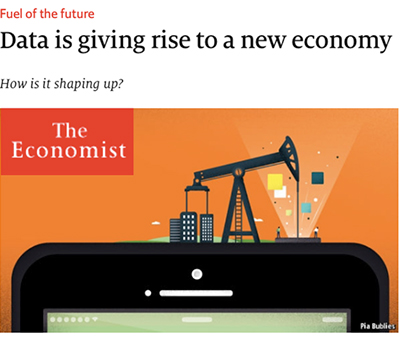
\includegraphics[scale=0.5]{figure/oil.jpg}

\end{frame}



\begin{frame}{Danger\footnote{\scriptsize\url{https://timoelliott.com/blog/2018/03/data-is-the-new-oil-yes-toxic-if-mishandled.html}}}
	\centering
	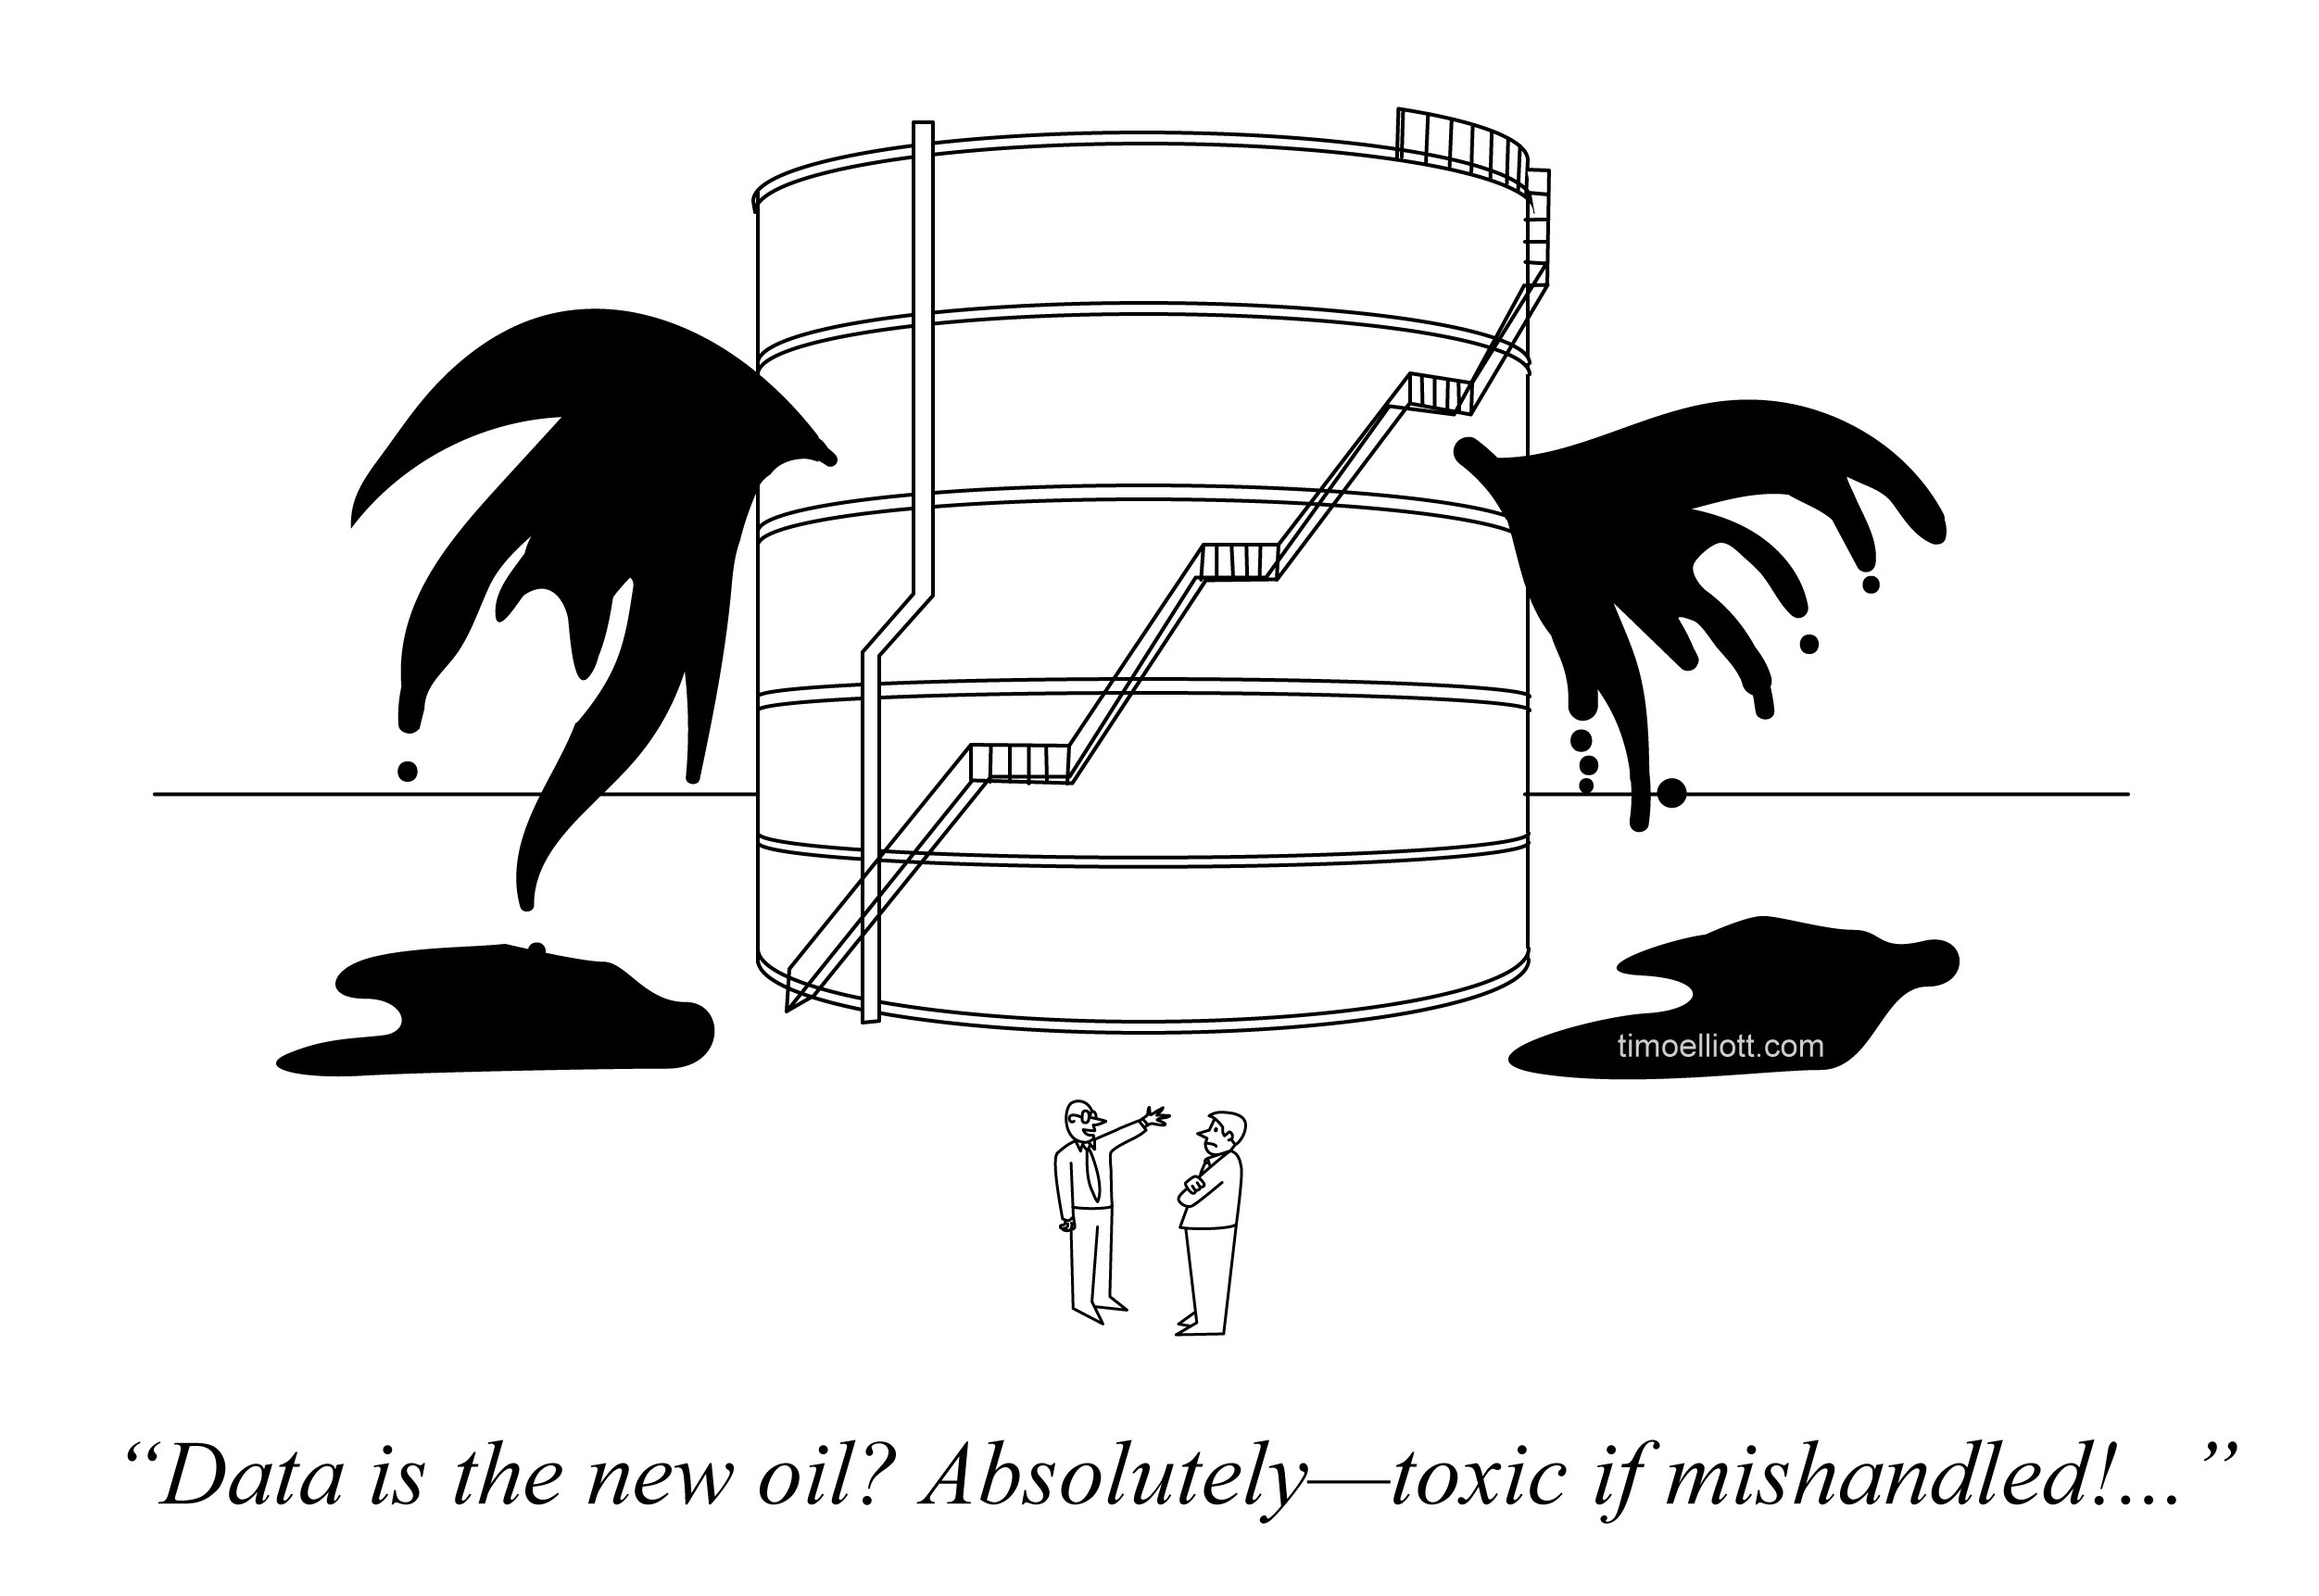
\includegraphics[scale=0.15]{figure/toxic.jpg}	
\end{frame}


\begin{frame}{Data science\footnote{\scriptsize\url{https://hbr.org/2012/10/data-scientist-the-sexiest-job-of-the-21st-century}}}
	\centering
	
\includegraphics[scale=0.35]{figure/hbr.png}	
\end{frame}



\begin{frame}{Why \texttt{R} ?}
	\Wider[9em]{
		\begin{figure}
			\begin{minipage}[h]{0.40\linewidth}
				\centering
				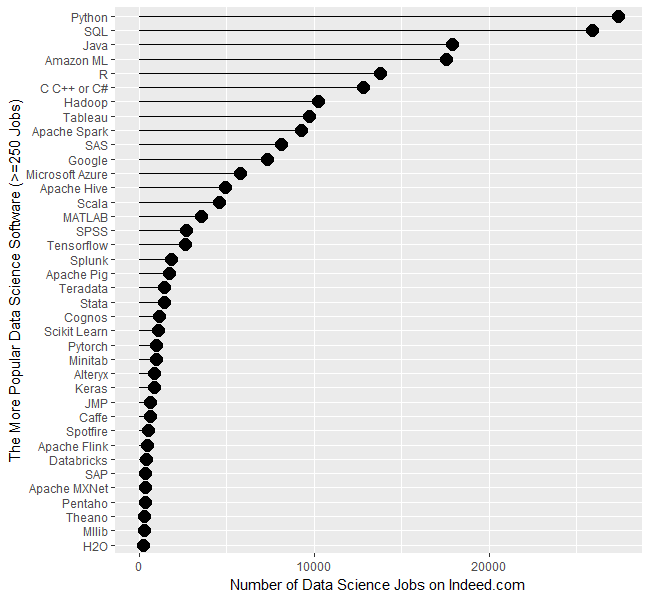
\includegraphics[scale=0.3]{figure/rjobs.png}
				\caption{Data as of May 2019 {\tiny \url{http://r4stats.com/articles/popularity/}}}
				\label{fig:a}
			\end{minipage}
			%\hspace{0.5cm}
			\begin{minipage}[h]{0.40\linewidth}
				\centering
				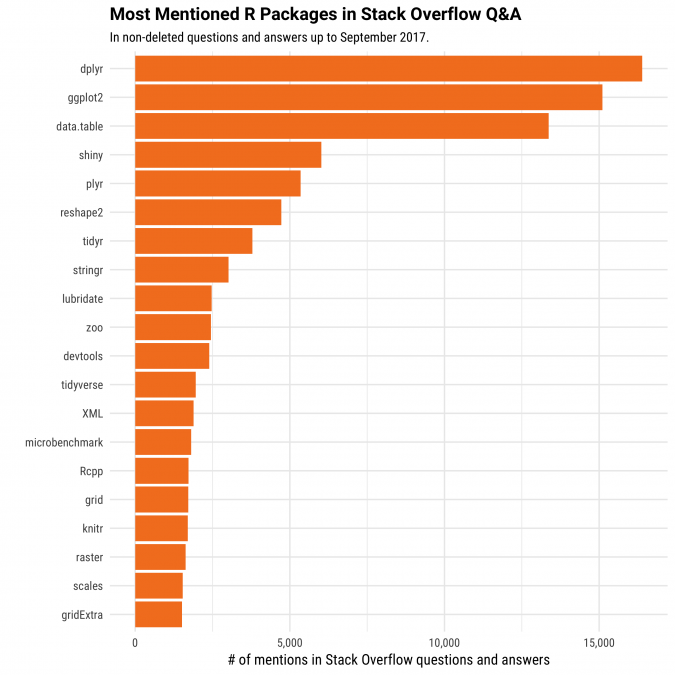
\includegraphics[scale=0.2]{figure/dplyr.png}
				\caption{Popular \texttt{R} packages {\tiny \url{https://stackoverflow.blog/2017/10/10/impressive-growth-r/}}}
				\label{fig:b}
			\end{minipage}
		\end{figure}
	}
\end{frame}


\begin{frame}{First day in a statistics course}
\Wider[5em]{
	\centering
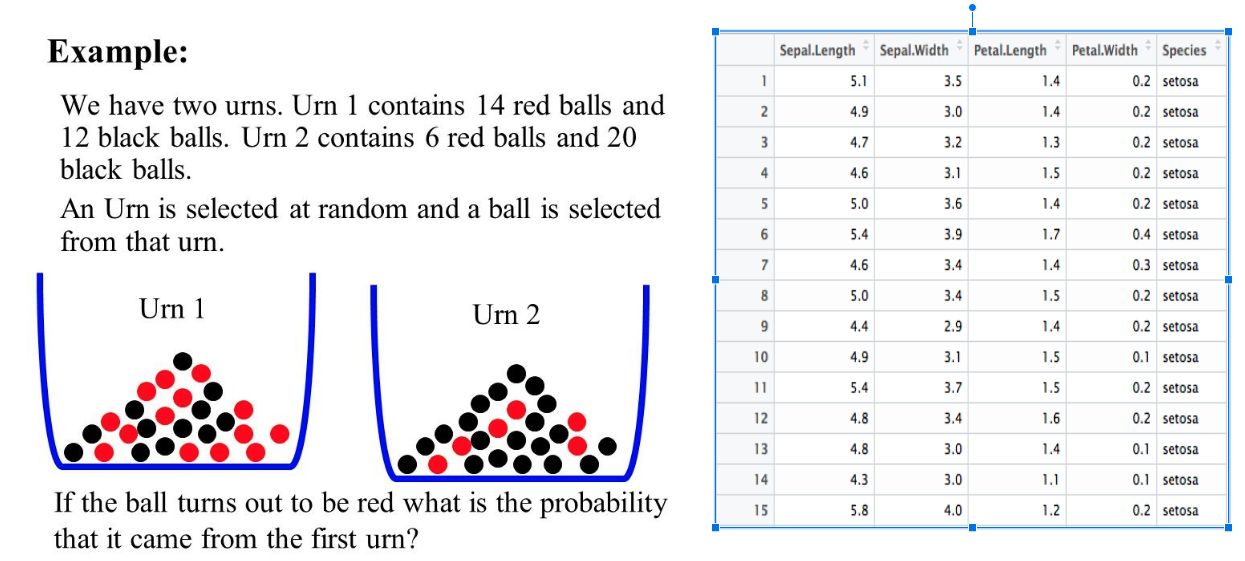
\includegraphics[scale=0.35]{figure/firstday.png}
}
\end{frame}


\begin{frame}{Second day in a statistics course}
	\Wider[5em]{
		\centering
		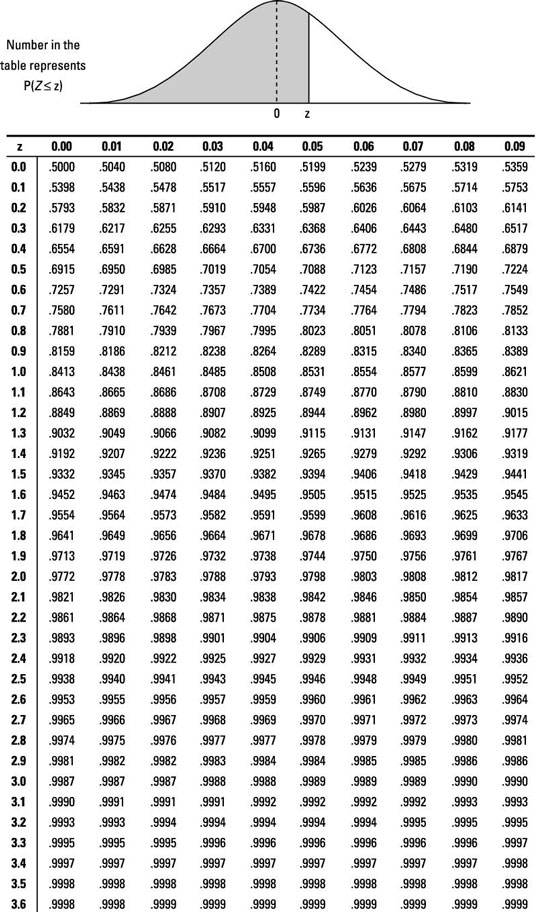
\includegraphics[scale=0.25]{figure/ztable.jpg}
	}
\end{frame}

\section{Gather data into analysis ready format}

\begin{frame}{Tidy data}
	
\begin{itemize}
	\setlength\itemsep{.51em}
	\item Each variable forms a column.
	\item Each observation forms a row.
	\item Each type of observational units forms a table
	\item Tidy data is ready for regression routines and plotting
\end{itemize}


\framedgraphic{figure/tidy.png}
\end{frame}



\begin{frame}[fragile]{Example: Does a full moon affect behaviour?}
	
	\small
	\begin{itemize}
		\item Many people believe that the moon influences the actions of some individuals. 
		\item A study of dementia patients in nursing homes recorded various types of disruptive behaviors every day for 12 weeks. 
		\item Days were classified as moon days if they were in a 3-day period centered at the day of the full moon. 
		\item For each patient, the average number of disruptive behaviors was computed for moon days and for all otherdays. 
	\end{itemize}
	
\begin{knitrout}\footnotesize
\definecolor{shadecolor}{rgb}{0.969, 0.969, 0.969}\color{fgcolor}
\begin{tabular}{r|r|r}
\hline
patient & moon\_days & other\_days\\
\hline
1 & 3.33 & 0.27\\
\hline
2 & 3.67 & 0.59\\
\hline
3 & 2.67 & 0.32\\
\hline
4 & 3.33 & 0.19\\
\hline
5 & 3.33 & 1.26\\
\hline
6 & 3.67 & 0.11\\
\hline
7 & 4.67 & 0.30\\
\hline
\end{tabular}


\end{knitrout}
	
	
	
\end{frame}


\begin{frame}[fragile]{Is it tidy?}
	
\begin{knitrout}\footnotesize
\definecolor{shadecolor}{rgb}{0.969, 0.969, 0.969}\color{fgcolor}
\begin{tabular}{r|r|r}
\hline
patient & moon\_days & other\_days\\
\hline
1 & 3.33 & 0.27\\
\hline
2 & 3.67 & 0.59\\
\hline
3 & 2.67 & 0.32\\
\hline
\end{tabular}


\end{knitrout}
	
	\pause
	
	\vspace*{0.4cm}
	
	\textcolor{blue}{\textbf{Question: Can I plot the data?}}
	
	\pause
	
\begin{knitrout}\tiny
\definecolor{shadecolor}{rgb}{0.969, 0.969, 0.969}\color{fgcolor}
\begin{alltt}
\hlkwd{plot}\hlstd{(df}\hlopt{$}\hlstd{moon_days, df}\hlopt{$}\hlstd{other_days,} \hlkwc{pch} \hlstd{=} \hlnum{19}\hlstd{)}
\hlkwd{abline}\hlstd{(}\hlkwc{a}\hlstd{=}\hlnum{0}\hlstd{,}\hlkwc{b}\hlstd{=}\hlnum{1}\hlstd{)}
\end{alltt}


{\centering 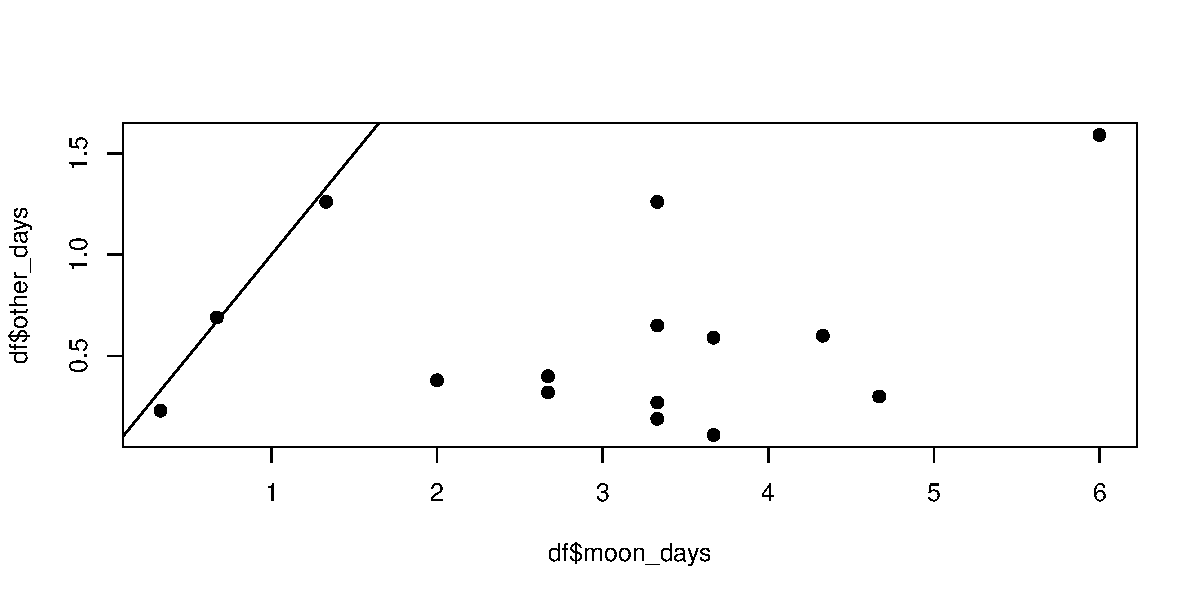
\includegraphics[width=1\linewidth]{figure/unnamed-chunk-3-1} 

}



\end{knitrout}
\end{frame}


\begin{frame}[fragile]{Is it tidy?}
	
\begin{knitrout}\footnotesize
\definecolor{shadecolor}{rgb}{0.969, 0.969, 0.969}\color{fgcolor}
\begin{tabular}{r|r|r}
\hline
patient & moon\_days & other\_days\\
\hline
1 & 3.33 & 0.27\\
\hline
2 & 3.67 & 0.59\\
\hline
3 & 2.67 & 0.32\\
\hline
4 & 3.33 & 0.19\\
\hline
5 & 3.33 & 1.26\\
\hline
\end{tabular}


\end{knitrout}
	
	\pause
	
	\vspace*{0.4cm}
	
	\textcolor{blue}{\textbf{Question: Can I fit a \underline{meaningful} regression model \underline{directly} to the \underline{variables} in the data?}}
	
	\pause
	
\begin{knitrout}\scriptsize
\definecolor{shadecolor}{rgb}{0.969, 0.969, 0.969}\color{fgcolor}
\begin{verbatim}
## Call: lm(formula = moon_days ~ other_days, data = df)
## 
## Coefficients:
##             Estimate Std. Error t value Pr(>|t|)
## (Intercept)     2.56       0.66     3.9    0.002
## other_days      0.79       0.91     0.9    0.402
## 
## Residual standard error: 1.5 on 13 degrees of freedom
## Multiple R-squared: 0.055,	Adjusted R-squared: -0.018 
## F-statistic: 0.75 on 1 and 13 DF,  p-value: 0.4
\end{verbatim}

\end{knitrout}
\end{frame}






\begin{frame}[fragile]{Is it tidy?}
	
\begin{knitrout}\footnotesize
\definecolor{shadecolor}{rgb}{0.969, 0.969, 0.969}\color{fgcolor}
\begin{tabular}{l|l|r}
\hline
patient & day\_type & mean\_behavior\\
\hline
1 & moon\_days & 3.33\\
\hline
1 & other\_days & 0.27\\
\hline
2 & moon\_days & 3.67\\
\hline
2 & other\_days & 0.59\\
\hline
3 & moon\_days & 2.67\\
\hline
3 & other\_days & 0.32\\
\hline
4 & moon\_days & 3.33\\
\hline
4 & other\_days & 0.19\\
\hline
5 & moon\_days & 3.33\\
\hline
5 & other\_days & 1.26\\
\hline
\end{tabular}


\end{knitrout}
	
	
\end{frame}


\begin{frame}[fragile]{Plotting with tidy data}
	
\begin{knitrout}\tiny
\definecolor{shadecolor}{rgb}{0.969, 0.969, 0.969}\color{fgcolor}
\begin{alltt}
\hlkwd{ggplot}\hlstd{(}\hlkwc{data} \hlstd{= df_tidy,} \hlkwc{mapping} \hlstd{=} \hlkwd{aes}\hlstd{(}\hlkwc{x} \hlstd{= day_type,} \hlkwc{y} \hlstd{= mean_behavior,} \hlkwc{group} \hlstd{= patient))} \hlopt{+} \hlkwd{geom_line}\hlstd{()}
\end{alltt}

\end{knitrout}
	
\begin{knitrout}\tiny
\definecolor{shadecolor}{rgb}{0.969, 0.969, 0.969}\color{fgcolor}

{\centering 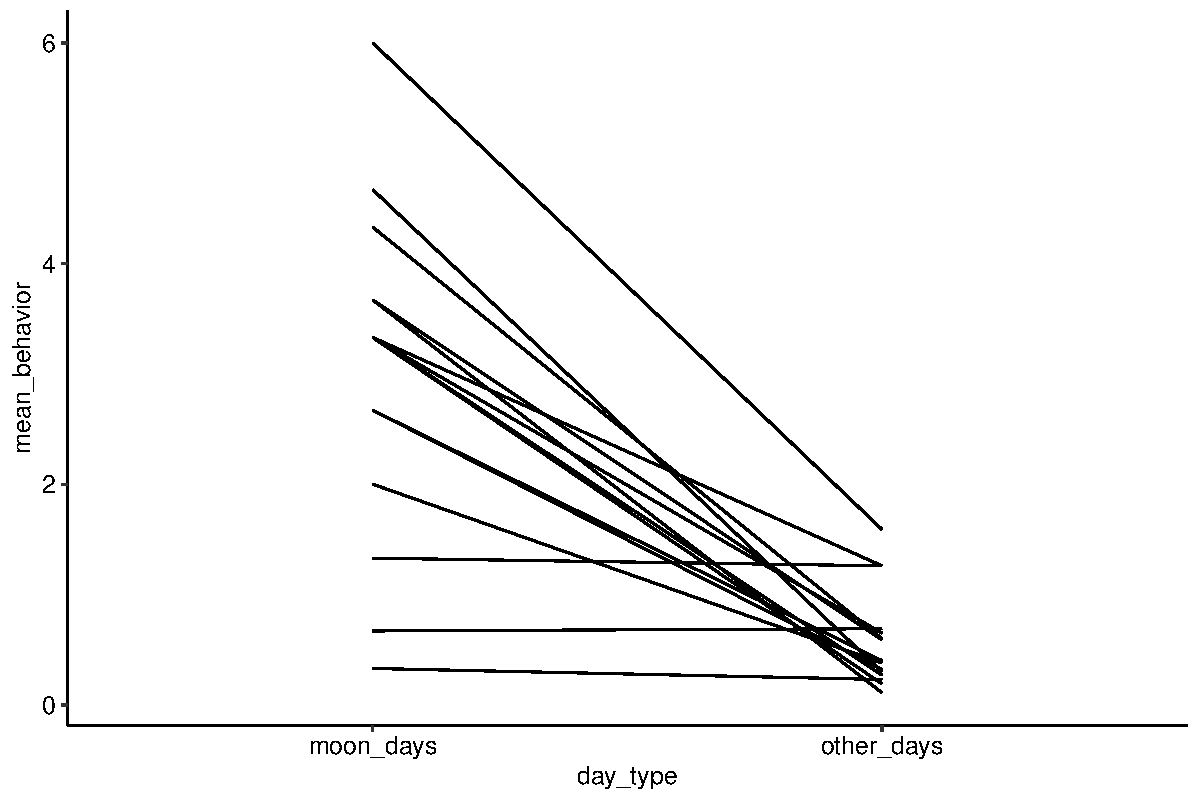
\includegraphics[width=1\linewidth]{figure/unnamed-chunk-8-1} 

}



\end{knitrout}
	
	
\end{frame}



\begin{frame}[fragile]{Regression with tidy data}
	
	
\begin{knitrout}\tiny
\definecolor{shadecolor}{rgb}{0.969, 0.969, 0.969}\color{fgcolor}
\begin{alltt}
\hlstd{fit} \hlkwb{<-} \hlstd{lme4}\hlopt{::}\hlkwd{lmer}\hlstd{(mean_behavior} \hlopt{~} \hlstd{day_type} \hlopt{+} \hlstd{(}\hlnum{1}\hlopt{|}\hlstd{patient),} \hlkwc{data} \hlstd{= df_tidy)}
\hlkwd{summary}\hlstd{(fit)}
\end{alltt}
\begin{verbatim}
## Linear mixed model fit by REML ['lmerMod']
## Formula: mean_behavior ~ day_type + (1 | patient)
##    Data: df_tidy
## 
## REML criterion at convergence: 90.3
## 
## Scaled residuals: 
##      Min       1Q   Median       3Q      Max 
## -2.27236 -0.30142 -0.04023  0.48540  2.44753 
## 
## Random effects:
##  Groups   Name        Variance Std.Dev.
##  patient  (Intercept) 0.1563   0.3954  
##  Residual             1.0659   1.0324  
## Number of obs: 30, groups:  patient, 15
## 
## Fixed effects:
##                    Estimate Std. Error t value
## (Intercept)          3.0220     0.2854  10.587
## day_typeother_days  -2.4327     0.3770  -6.453
## 
## Correlation of Fixed Effects:
##             (Intr)
## dy_typthr_d -0.660
\end{verbatim}

\end{knitrout}
\end{frame}



\begin{frame}[fragile]{Not tidy vs. tidy data}
	
	
	%\Wider[4em]{
	%\centering
	
	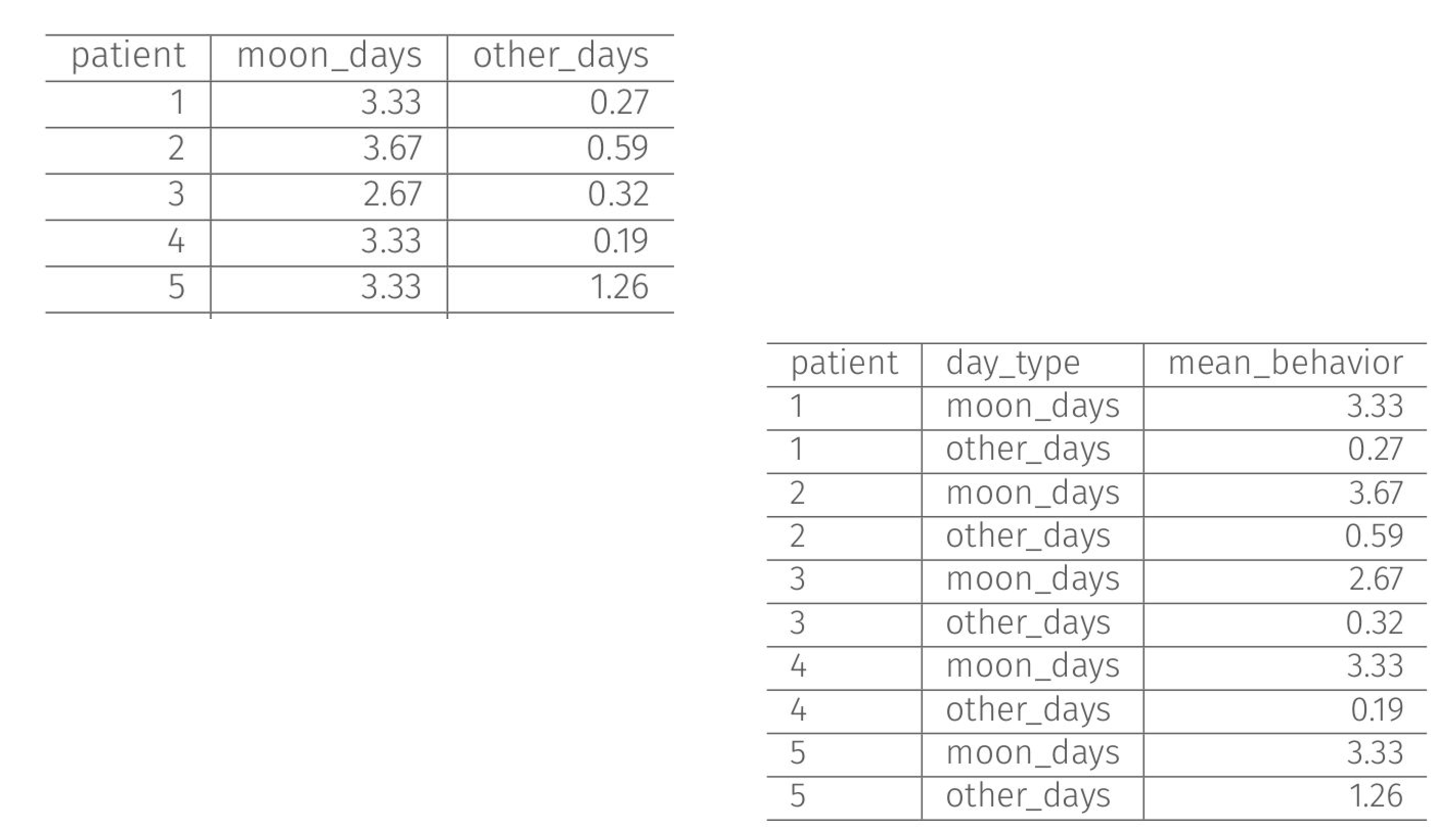
\includegraphics[scale=0.45]{figure/tidy3.pdf}
	
	
	%\framedgraphiccaption{tidy-fullmoon.jpg}{\texttt{text}}
	%}
	
\end{frame}

\begin{frame}[fragile]{Not tidy vs. tidy data}
	
	
	%\Wider[4em]{
	%\centering
	
	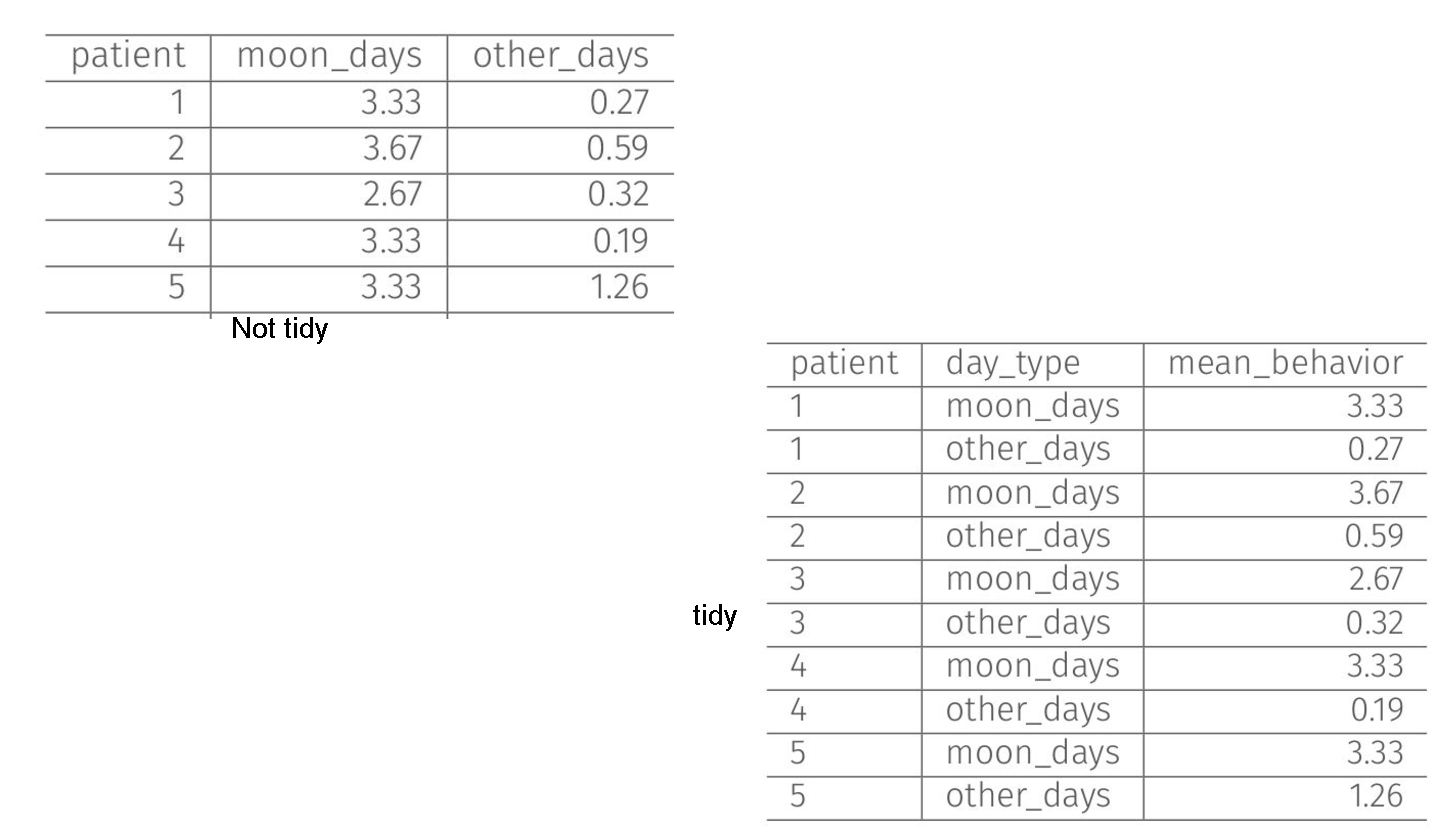
\includegraphics[scale=0.45]{figure/tidy4.pdf}
	
	
	%\framedgraphiccaption{tidy-fullmoon.jpg}{\texttt{text}}
	%}
	
\end{frame}







\begin{frame}[fragile]{\texttt{tidyr::pivot\_longer()}}
	
	
	%\Wider[4em]{
	%\centering
	
	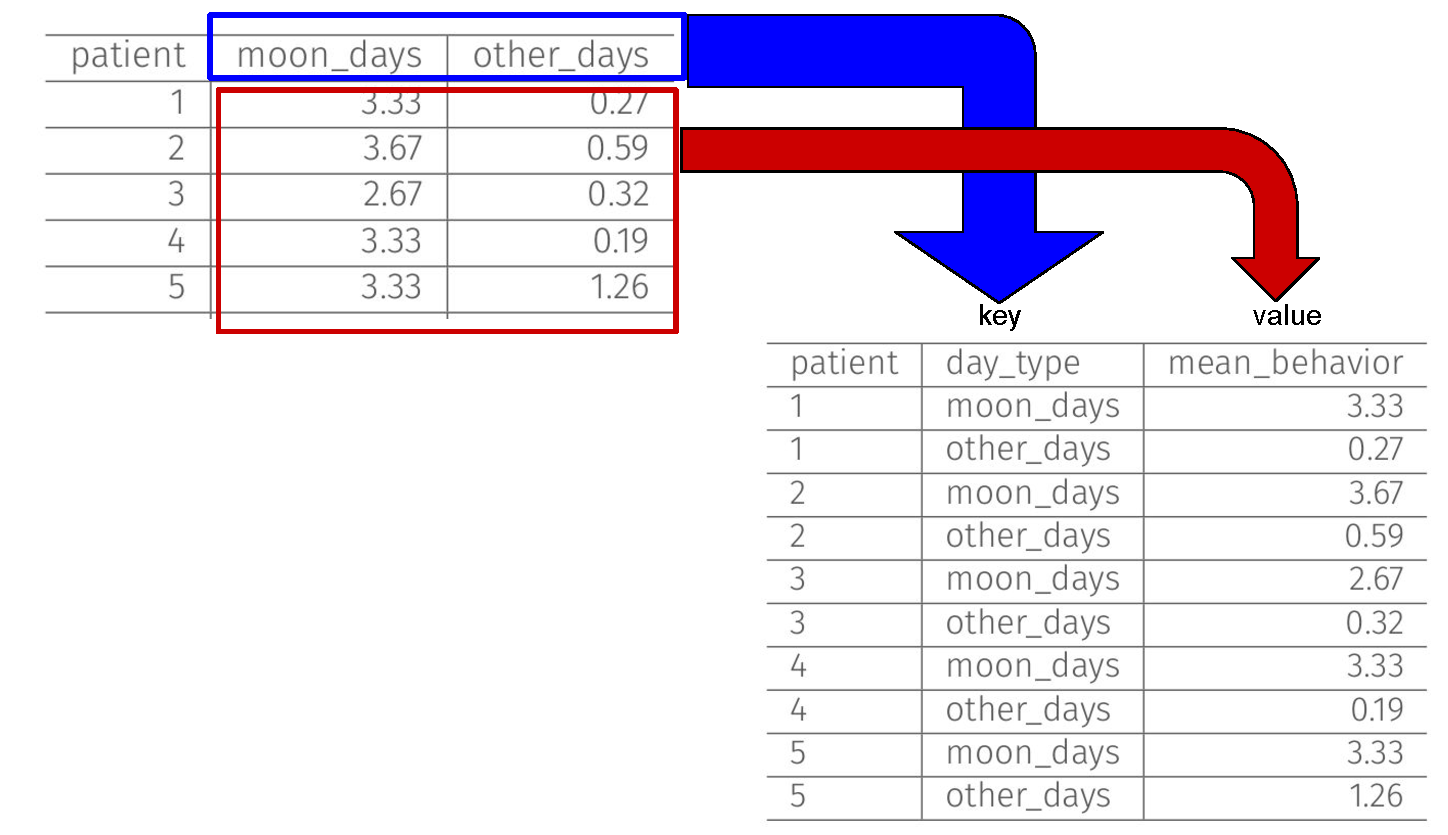
\includegraphics[scale=0.45]{figure/tidy1.pdf}
	
	%\pause
	
\begin{knitrout}\tiny
\definecolor{shadecolor}{rgb}{0.969, 0.969, 0.969}\color{fgcolor}
\begin{alltt}
\hlstd{tidyr}\hlopt{::}\hlkwd{pivot_longer}\hlstd{(}\hlkwc{data} \hlstd{= df,} \hlkwc{cols} \hlstd{=} \hlopt{-}\hlstd{patient,} \hlkwc{names_to} \hlstd{=} \hlstr{"day_type"}\hlstd{,} \hlkwc{values_to} \hlstd{=} \hlstr{"mean_behavior"}\hlstd{)}
\end{alltt}

\end{knitrout}
	
	%\framedgraphiccaption{tidy-fullmoon.jpg}{\texttt{text}}
	%}
	
\end{frame}



\section{Learn regression}


\begin{frame}{Traditional stats textbook}
	\Wider[4em]{
	\centering
	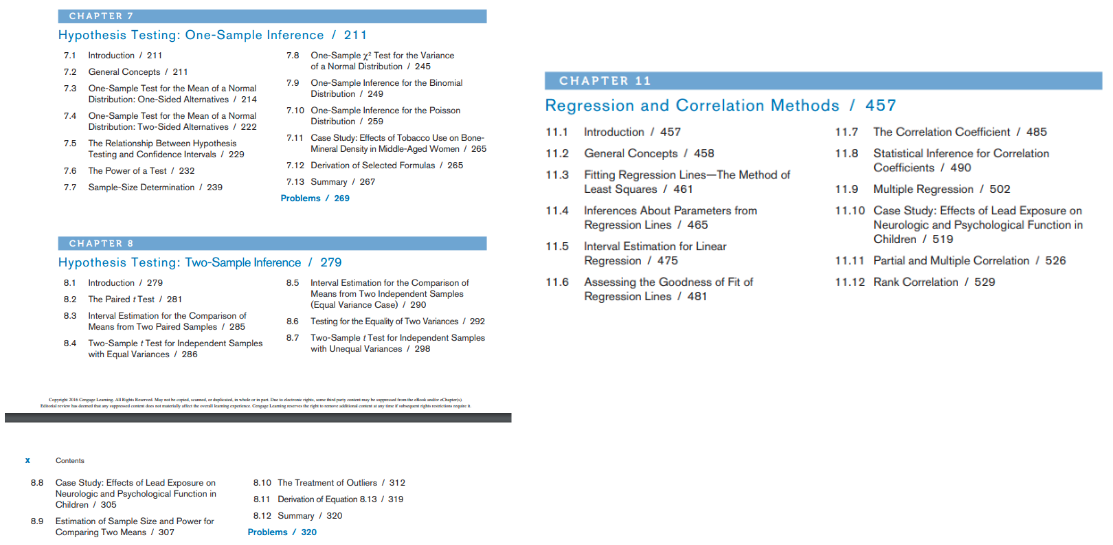
\includegraphics[scale=0.4]{figure/text1.png}
}
\end{frame}


\begin{frame}{This course}
		\Wider[4em]{
	\centering
	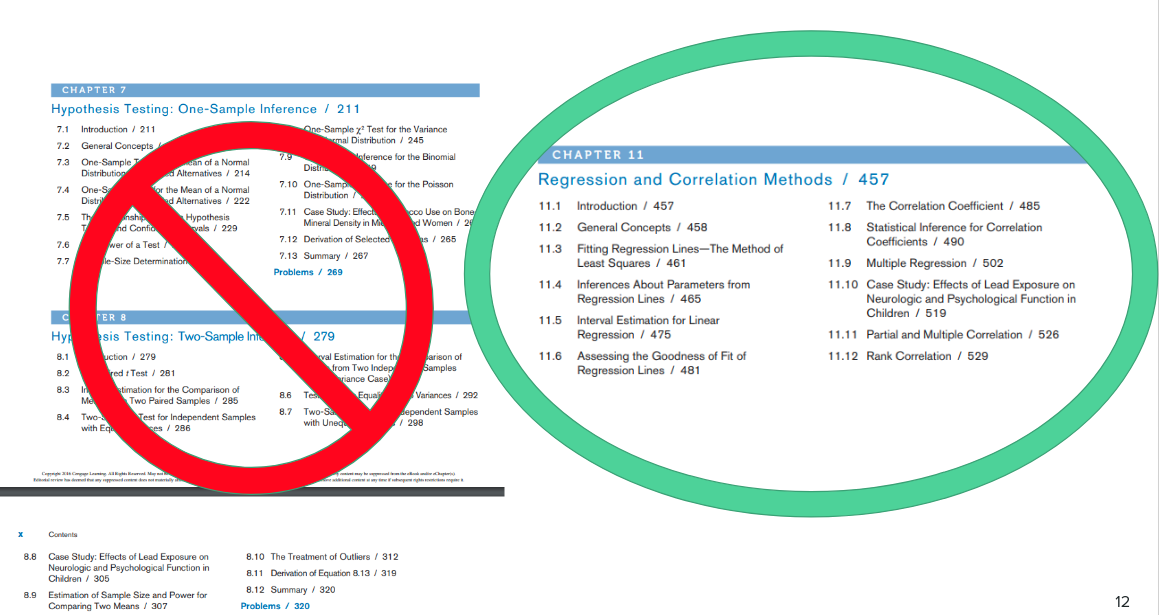
\includegraphics[scale=0.4]{figure/text2.png}
}
\end{frame}


\section{Understand the statistical results in a scientific paper}

\begin{frame}{Statistical concepts}
			\Wider[4em]{
		\centering
		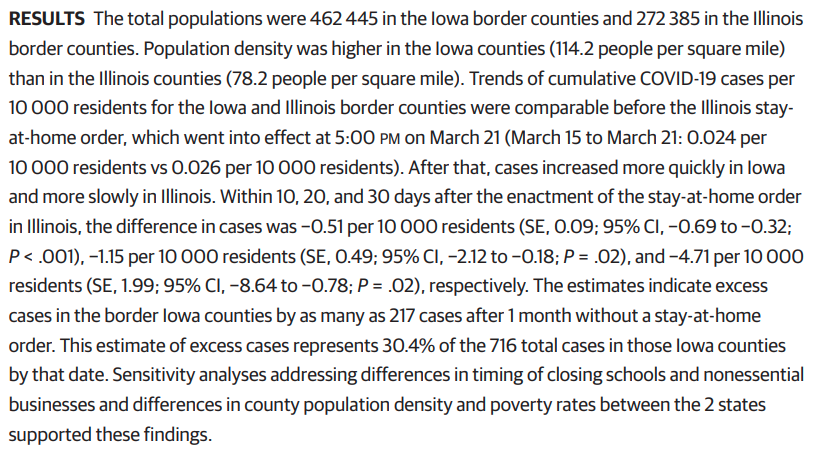
\includegraphics[scale=0.5]{figure/jama1.png}
	}
\footnote{\footnotesize \url{https://jamanetwork.com/journals/jamanetworkopen/fullarticle/2766229}}
\end{frame}


\begin{frame}{Statistical concepts}
	\Wider[4em]{
		\centering
		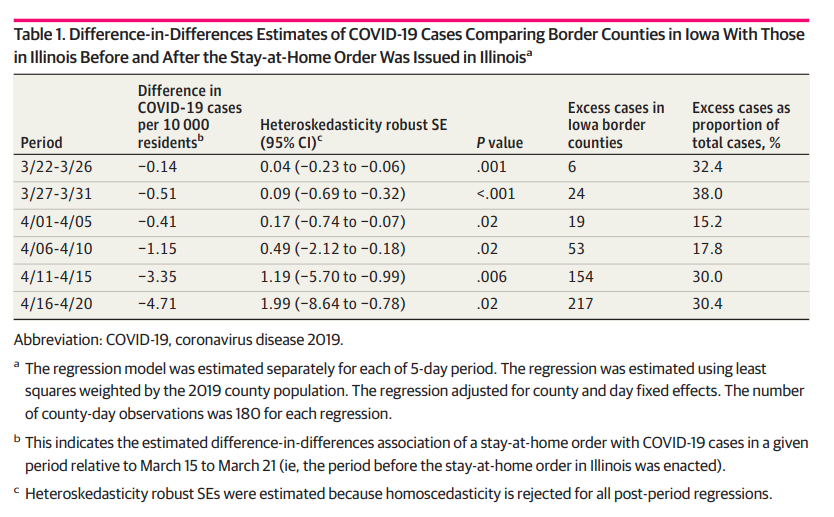
\includegraphics[scale=0.5]{figure/jama2.png}
	}
	\footnote{\footnotesize \url{https://jamanetwork.com/journals/jamanetworkopen/fullarticle/2766229}}
\end{frame}



\section{Learn the tools for creating reproducible analyses}


\begin{frame}{Copy paste ad nauseam}
		\Wider[4em]{
		\centering
		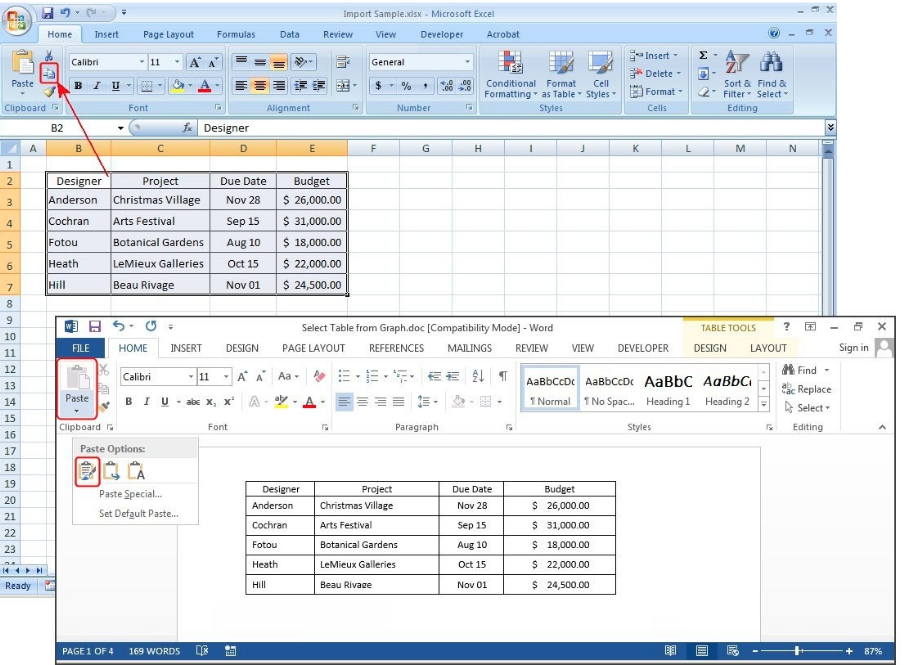
\includegraphics[scale=0.35]{figure/excel.png}
	}
\end{frame}


\begin{frame}{Markdown: HTML without knowing HTML}
	\begin{center}
		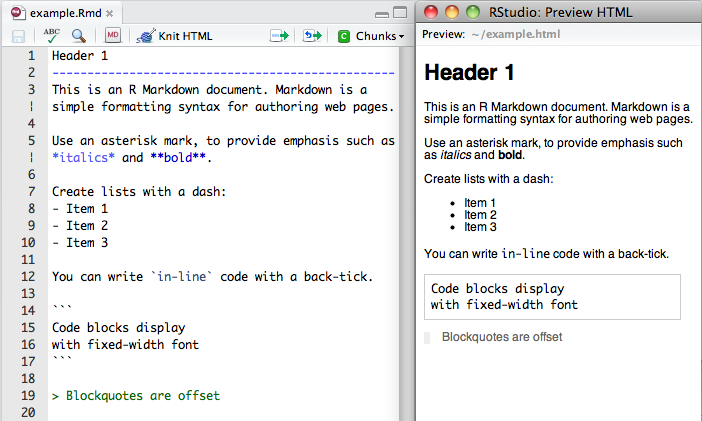
\includegraphics[scale=0.45, keepaspectratio]{figure/markdown}
	\end{center}
\end{frame}

\begin{frame}{R + Markdown = RMarkdown}
	\begin{center}
		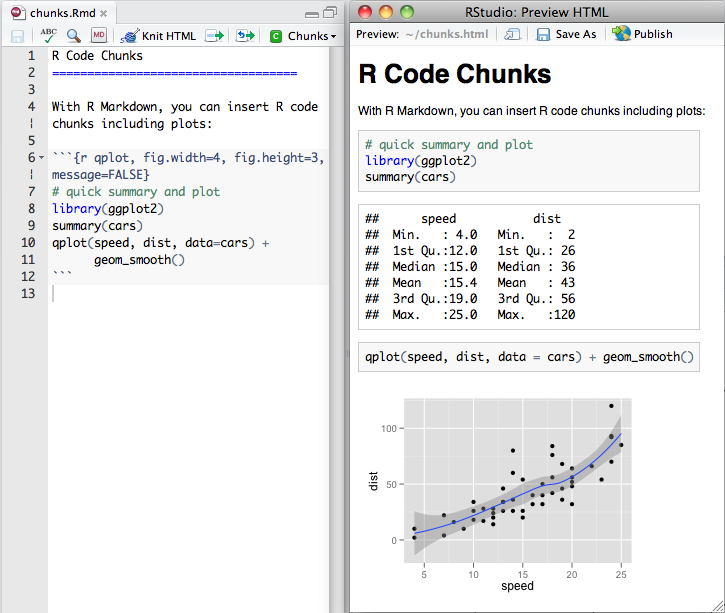
\includegraphics[scale=0.36, keepaspectratio]{figure/rmarkdown}
	\end{center}
\end{frame}

\begin{frame}{What \texttt{rmarkdown} does}
	\textbf{\code{RMarkdown}} example:
	
	\begin{center}
		\begin{tikzpicture}
		\scriptsize
		\node (expr) [startstop] {Report.Rmd (contains both code and markdown)};
		\node (science) [decision, below of=expr, xshift=0cm, yshift=-2cm] {Report.md};
		\draw [arrow] (expr) -- node[anchor=east]{\texttt{knitr::knit('Report.Rmd')}} (science);
		\pause \node (pdf) [io, below of=science, xshift=0cm, yshift=-2cm] {Report.html, Report.pdf, Report.doc};
		\draw [arrow] (science) -- node[anchor=east]{\texttt{pandoc}} (pdf);
		\end{tikzpicture}
	\end{center}
\end{frame}


\begin{frame}\frametitle{Compiling a \texttt{.Rmd} document}
	
	\begin{block}{The two steps on previous slide can be executed in one command:}
		\[ \textrm{\texttt{rmarkdown::render()}} \]
	\end{block}
	
	or in \texttt{RStudio}:
	\begin{figure}[h!]
		\centering
		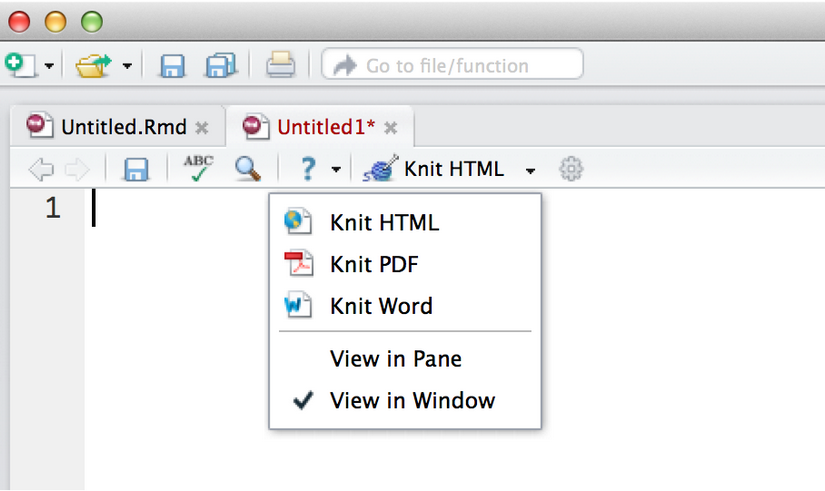
\includegraphics[scale=0.21, keepaspectratio]{figure/rmddrop.png}
	\end{figure}
	%\textit{Demonstrate:} Explore \texttt{RStudio}, projects and \texttt{.Rprofile}
\end{frame}


\section{Where does this course fit in my life?}

\begin{frame}{Topics by level of exposure}
			\Wider[4em]{
	\centering
	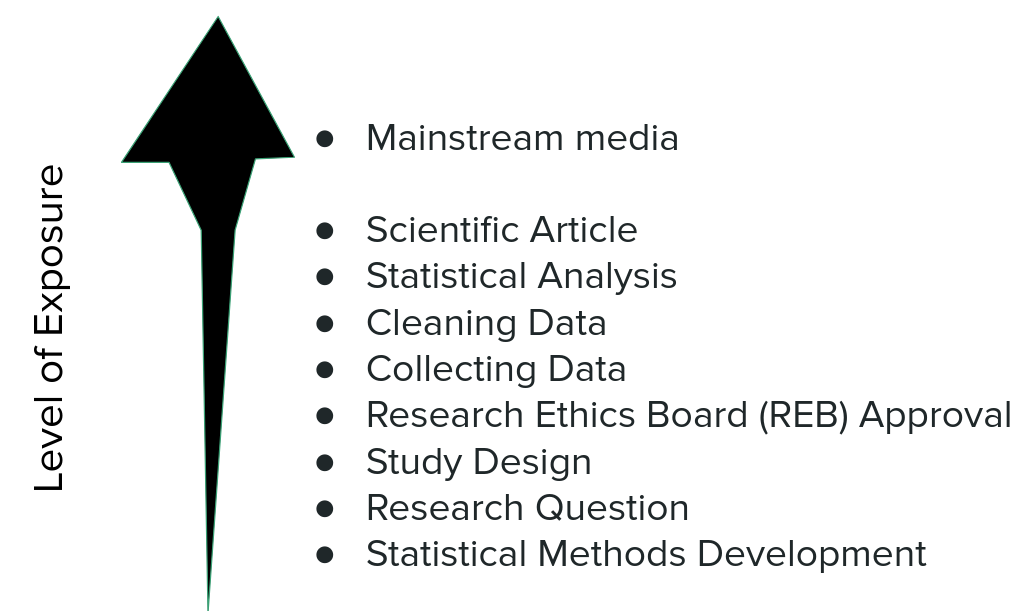
\includegraphics[scale=0.45]{figure/persp1.png}
}
\end{frame}

\begin{frame}{First year courses}
	\Wider[4em]{
		\centering
		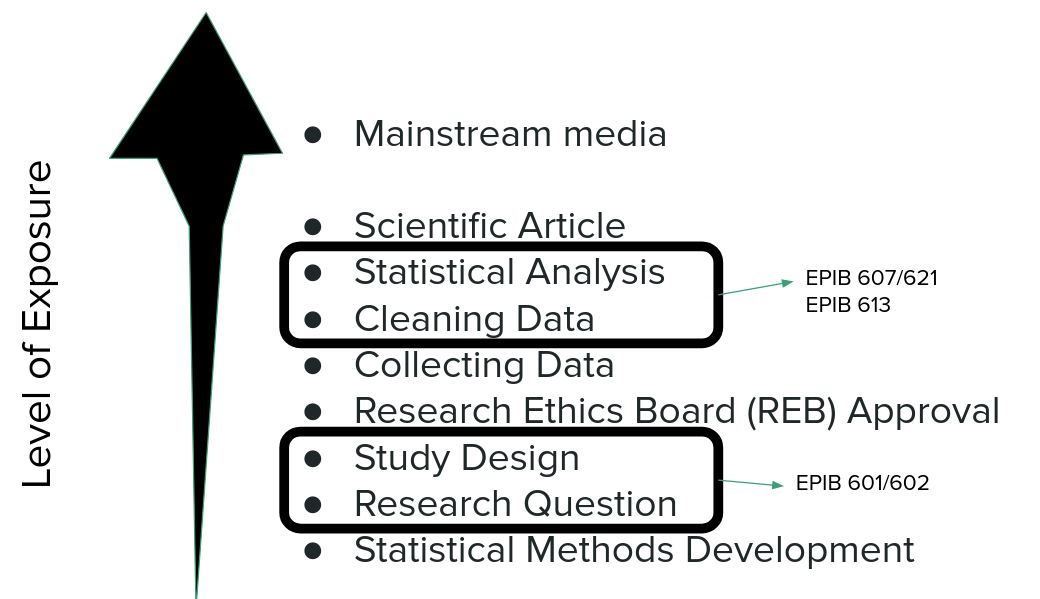
\includegraphics[scale=0.45]{figure/persp2.png}
	}
\end{frame}


\begin{frame}{My area of research}
	\Wider[4em]{
		\centering
		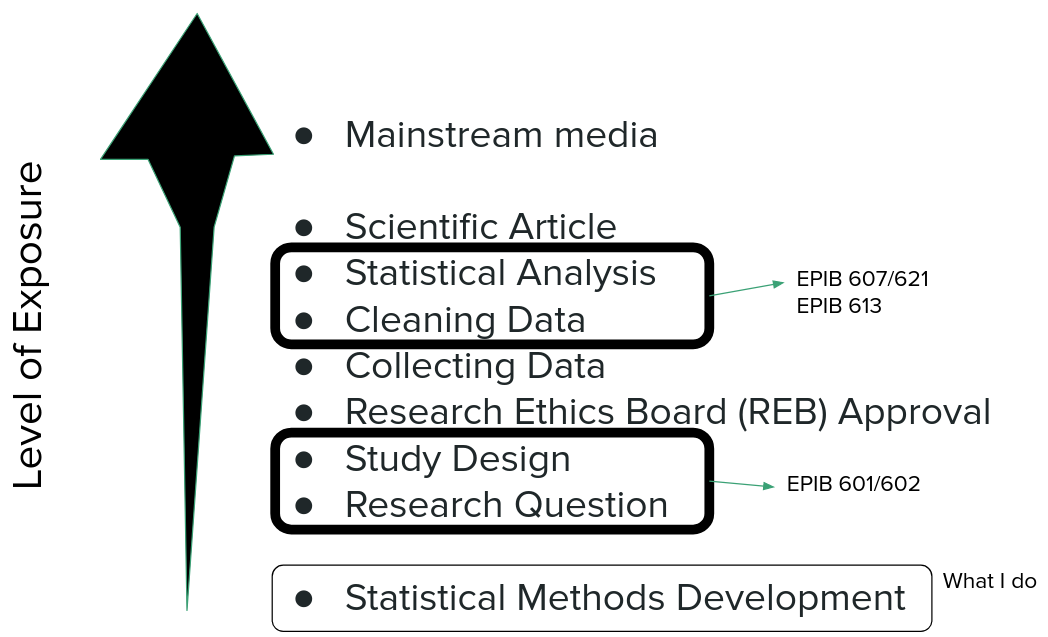
\includegraphics[scale=0.45]{figure/persp3.png}
	}
\end{frame}

%\begin{frame}[allowframebreaks]
%\nocite{breiman1984classification}
%	\nocite{friedman2001elements}
%	\nocite{james2013introduction}
%	\nocite{lopez2015arbres}
%	\frametitle{References}
%\printbibliography
%\end{frame}


\begin{frame}[fragile]{Session Info}
	\tiny
	
\begin{knitrout}\tiny
\definecolor{shadecolor}{rgb}{0.969, 0.969, 0.969}\color{fgcolor}
\begin{verbatim}
R version 3.6.2 (2019-12-12)
Platform: x86_64-pc-linux-gnu (64-bit)
Running under: Pop!_OS 19.10

Matrix products: default
BLAS:   /usr/lib/x86_64-linux-gnu/openblas/libblas.so.3
LAPACK: /usr/lib/x86_64-linux-gnu/libopenblasp-r0.3.7.so

attached base packages:
[1] stats     graphics  grDevices utils     datasets  methods   base     

other attached packages:
 [1] NCStats_0.4.7      FSA_0.8.30         forcats_0.5.0      stringr_1.4.0     
 [5] dplyr_1.0.2        purrr_0.3.4        readr_1.3.1        tidyr_1.1.2       
 [9] tibble_3.0.3       ggplot2_3.3.2.9000 tidyverse_1.3.0    knitr_1.29        

loaded via a namespace (and not attached):
 [1] Rcpp_1.0.4.6       lubridate_1.7.4    lattice_0.20-38    assertthat_0.2.1  
 [5] digest_0.6.25      R6_2.4.1           cellranger_1.1.0   plyr_1.8.6        
 [9] backports_1.1.9    reprex_0.3.0       evaluate_0.14      httr_1.4.1        
[13] highr_0.8          pillar_1.4.6       TeachingDemos_2.12 rlang_0.4.7       
[17] readxl_1.3.1       rstudioapi_0.11    minqa_1.2.4        nloptr_1.2.2.1    
[21] Matrix_1.2-18      labeling_0.3       splines_3.6.2      lme4_1.1-21       
[25] munsell_0.5.0      broom_0.7.0        compiler_3.6.2     modelr_0.1.5      
[29] xfun_0.16          pkgconfig_2.0.3    tidyselect_1.1.0   fansi_0.4.1       
[33] crayon_1.3.4       dbplyr_1.4.2       withr_2.2.0        ggpubr_0.2.5      
[37] MASS_7.3-51.5      grid_3.6.2         nlme_3.1-143       jsonlite_1.7.0    
[41] gtable_0.3.0       lifecycle_0.2.0    DBI_1.1.0          magrittr_1.5      
[45] scales_1.1.1       cli_2.0.2          stringi_1.4.6      farver_2.0.3      
[49] ggsignif_0.6.0     fs_1.3.2           xml2_1.3.0         ellipsis_0.3.1    
[53] generics_0.0.2     vctrs_0.3.4        boot_1.3-24        tools_3.6.2       
[57] glue_1.4.2         hms_0.5.3          colorspace_1.4-1   rvest_0.3.5       
[61] haven_2.3.1       
\end{verbatim}

\end{knitrout}

\end{frame}

\end{document}
